\chapter{Features}
Uno de los mayores desafios de Vulkan es ofrecer un alto rendimiento del hardware, con el menor consumo y calentamiento
que sea posible. Actualmente los dispositivos móviles tienen la posiblidad de ejecutar juegos con una gran calidad
gráfica. Uno de los métodos que se emplea es un menor uso de la \gls{cpu}, delegando menos tareas a esta y dando a la
\gls{gpu} una mayor responsabilidad sobre la ejecución: uso de lotes de tareas para ejecutar las tareas en la
\gls{gpu}, y empleo exclusivo de la \gls{cpu} para realizar rendering y computación.

El llegar a todos los dispositivos es otro de los objetivos centrales. Vulkan está disponible en Windows 7, Windows 8,
Windows 10, Tizen, GNU/Linux y Android. El kit de desarrollo está disponible tanto para sistemas de escritorio Windows
como para GNU/Linux. En Mac OS se está desarrollando una solución por parte de terceros para conseguir ejecutar
aplicaciones Vulkan. The Brenwill Workshop es una desarrolladora especializada en software gráfico que se ha propuesto
crear un wrapper entre las \gls{api} OpenGL y Metal para conseguir el soporte de Vulkan en MacOS e iOS. La solución
se llama MoltenVK, y es parte de un framework para desarrollo gráfico.

Vulkan implementa varias mejoras a nivel técnico las cuales le dan un buen motivo para ser el sucesor de OpenGL:
\begin{enumerate}
    \item Escalado en \gls{cpu}s multicore de forma nativa.
    \item Uso de binarios intermedios SPIR-V: Vulkan genera su propio código para shaders, de forma que los drivers no
    requieren del desarrollo de un propio compilador para poder renderizarlas. Al poder estar precompiladas, se puede
    emplear un mayor rango de shaders por escena. El driver tan solo se encarga de realizar optimizaciones y la
    generación de código final.
    \item Gestión unificada de kernels de cómputo y shaders gráficos: se juntan las dos API que hasta ahora estaban
    separadas.
    \item Orientado a objetos, no hay un estado global.
    \item Los estados no se encuentran atados a un contexto, se cachean en un buffer.
    \item Se puede emplear multithreading.
    \item Control sobre la memoria y la sincronización.
\end{enumerate}

Hay características que aún estan propuestas para su implantación, como por ejemplo el soporte de múltiples \gls{gpu}s
a la vez de diferente modelo. Se elimina la necesidad de SLI y Crossfire para poder emplear varias tarjetas gráficas al
mismo tiempo.

En la imagen \ref{fig:comparison_opengl_vulkan} se puede apreciar más gráficamente las diferencias que hay entre las
dos \gls{api}. Como se ha podido apreciar entre las características de Vulkan, se ha intentado que las aplicaciones
tengan un acceso más cercano al hardware. Gracias a esto se elimina la necesidad de una gran gestión de errores
y de memoria. Tan solo se emplea un lenguaje intermedio para los shaders (SPIR-V), y la \gls{api} es la misma tanto
para desarrollar para dispostivos móviles como para aplicaciones de escritorio.

Con toda esta información podría parecer que Vulkan aumenta la carga de trabajo que tienen los desarrolladores, aunque
las cosas no son como parecen. Se puede implementar Vulkan a tres niveles diferentes: (1) usar directamente todas las
prestaciones para tener control total sobre el motor, (2) emplear librerías y capas para acelerar el desarrollo, o
(3) emplear motores optimizados sobre la \gls{api} Vulkan. La primera opción es la que menor uso va a tener, pero puede
ser una buena opción para realizar bencharmarks. Khronos espera que la segunda opción sea una rica área de innovación
ya que las librerías pueden ser OpenSource que requieran de mejoras y actualizaciones. La última opción puede ser la
más tentativa, ya que el trabajo más duro ya ha sido realizado por los gigantes de la industria.

En la imagen \ref{fig:vulkan_ecosystem} puede apreciarse como se distribuye la arquitectura de Vulkan. Como se ha
explicado, Vulkan se situa en un nivel inferior al motor del juego. Se sitúa justo encima del hardware, por lo que
se puede explotar muchas de sus características directamente. Se habilita una interfaz para poder implementar en el
futuro otras herramientas y frameworks para usar conjuntamente con Vulkan.

\begin{figure}[t]
	\begin{center}
		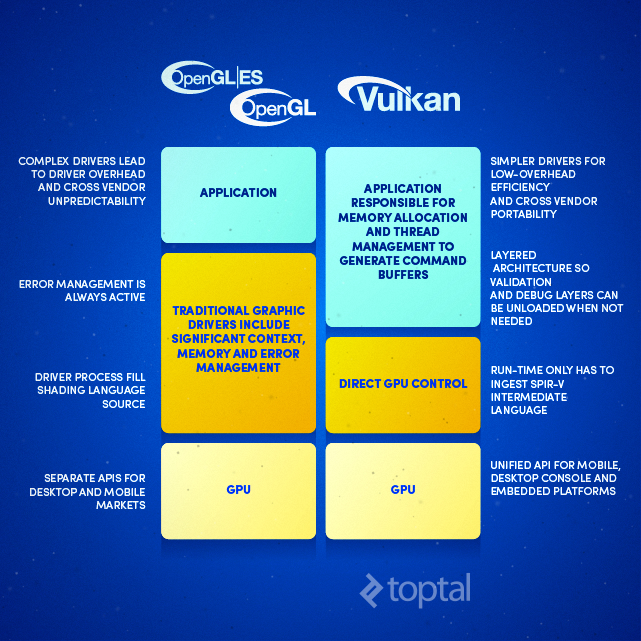
\includegraphics[scale=0.3]{comparison-opengl_and_vulkan}
		\caption{Comparativa entre características de OpenGL y Vulkan}
		\label{fig:comparison_opengl_vulkan}
	\end{center}
\end{figure}
\begin{figure}[t]
	\begin{center}
		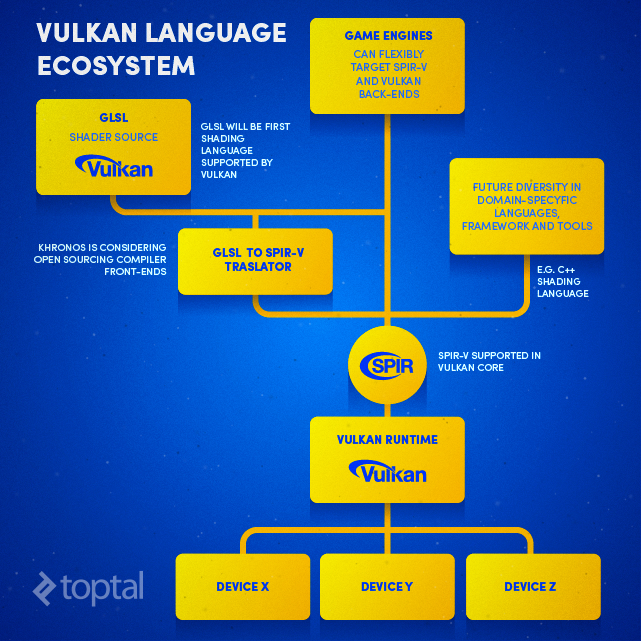
\includegraphics[scale=0.3]{ecosystem-vulkan}
		\caption{Ecosistema Vulkan}
		\label{fig:vulkan_ecosystem}
	\end{center}
\end{figure}
